 \documentclass[a4paper,12pt]{article} 
\usepackage[T2A]{fontenc}			
\usepackage[utf8]{inputenc}			
\usepackage[english,russian]{babel}	
\usepackage{amsmath,amsfonts,amssymb,amsthm,mathrsfs,mathtools} 
\usepackage[colorlinks, linkcolor = purple, citecolor = purple]{hyperref}
\usepackage{xcolor}
\usepackage{xpatch}
\usepackage{marvosym}
\usepackage{cancel}
\usepackage{floatrow}
\usepackage{commath}
\usepackage{upgreek}
\usepackage{lipsum}
\usepackage{mhchem}
\usepackage{chemfig}
\usepackage{multirow}
\usepackage{tikz}
\usepackage{titletoc}
\usepackage{pgfplots}
\usepackage{wrapfig}
\usepackage{chngcntr}
\usepackage{makecell}
\usepackage{stackengine,graphicx}
\usepackage{cmap}
\usepackage{indentfirst}
\usepackage{tocloft}
\usepackage{setspace}
\usepackage{titlesec}
\usepackage{soul}
\usepackage[stable]{footmisc}
\usepackage{tocloft}
\usetikzlibrary{positioning}
\usepackage{caption}
\usepackage{subfig}
\pgfplotsset{width=10cm,compat=1.9}
\tikzset{>=stealth}
\usepackage[left=2cm,right=2cm,top=2cm,bottom=3cm,bindingoffset=0cm]{geometry}
%\DeclareMathOperator*{\esssup}{ess\,sup}
\DeclareMathOperator*{\tr}{tr}
\DeclareMathOperator*{\Ker}{Ker}
\DeclareMathOperator*{\Rea}{Re}
\DeclareMathOperator*{\Ima}{Im}
\DeclareFontEncoding{LS2}{}{\noaccents@}
\DeclareFontSubstitution{LS2}{stix}{m}{n}
\DeclareSymbolFont{arrows3}{LS2}{stixtt}{m}{n}
\DeclareMathSymbol{\squareulblack}{\mathord}{arrows3}{"88}
\date{\vspace{-10pt}}
\author{Дорогинин Д.В. Б02-825бф\\
Матвеев Г.А. Б02-824бф}
\title{\textbf{Электронный парамагнитный резонанс.}}


\theoremstyle{definition}
\newtheorem*{definition}{Определение}
\newtheorem{statement}{Предложение}
\newtheorem{lemma}{Лемма}
\newtheorem{theorem}{Теорема}
\newtheorem*{theorem*}{Теорема}
\newtheorem*{corollary}{Следствие}
\newtheorem*{example}{Пример}
\setcounter{tocdepth}{2}
%\renewcommand\cftsecafterpnum{\vspace{-pt}}
%\renewcommand\cftsecafterpnum{\vspace{1pt}}
\newcommand*{\eqdef}{\mathop{\overset{\mathrm{def}}{\resizebox{\widthof{\ensuremath{\mathop{\overset{\mathrm{def}}{=}}}}}{\heightof{=}}{=}}}}
\renewcommand\qedsymbol{$\squareulblack$}
\renewcommand{\cftsecleader}{\cftdotfill{\cftdotsep}}
\newfloatcommand{capbtabbox}{table}[][\FBwidth]
\newcommand{\HH}{\mathcal{H}}
\newcommand{\DD}{\mathcal{D}}
\newcommand{\LL}{\mathcal{L}}
\newcommand{\AAA}{\mathscr{A}}
\newcommand{\SpA}{\mathcal{A}}
\newcommand{\EE}{\mathcal{E}}
\newcommand{\suml}{\sum\limits_{n=1}^\infty}
\newcommand{\sumlN}{\sum\limits_{n=1}^N}
\newcommand{\sumo}{\sum\limits_{n=0}^\infty}
\newcommand{\sumoN}{\sum\limits_{n=0}^N}
\renewcommand\cftsecfont{\normalsize}
\renewcommand\cftsubsecfont{\normalsize}
\titleformat{\section}
  {\normalfont\fontsize{16}{16}\bfseries}{\thesection}{1em}{}
\def\rlwd{.5pt}
\def\crossy{\kern.5pt\def\stacktype{L}%
 \stackon[0.65ex]{%
  \stackon[1.4ex]{%
    \stackon[1.1ex]{\rule{\rlwd}{1.8ex}}{\rule{1.4ex}{\rlwd}}%
  }{\rule{0.8ex}{\rlwd}}%
 }{\rotatebox{-20}{\rule{0.8ex}{\rlwd}}}%
\kern1pt}



\newcommand{\angstrom}{\mbox{\normalfont\AA}}


\begin{document}
\begin{titlepage}
	\begin{center}
		\large 	Московский физико-технический институт \\
		(национальный исследовательский университет) \\
		Факультет общей и прикладной физики \\
		\vspace{0.2cm}
		
		\vspace{4.5cm}
		Лабораторная работа №6.9.1  \\ \vspace{0.2cm}
		\large (Основы современной физики) \\ \vspace{0.2cm}
		\LARGE \textbf{ Закон Кюри--Вейса и обменное взаимодействие в
ферромагнетиках  }
	\end{center}
	\vspace{2.3cm} \large
	
	\begin{center}
		Работу выполнил: \\
		Дорогинин Демид,
		группа Б02-825
		\vspace{10mm}			
	\end{center}
		
	\begin{center} \vspace{60mm}
		г. Долгопрудный \\
		2021 год
	\end{center}
\end{titlepage}


\stepcounter{page}
\section*{Аннотация}
В работе исследуется температурная зависимость магнитной восприимчивости ферромагнетика в парамагнитной области -- выше точки Кюри. По полученной в работе температуре Кюри оценивается энергия обменного взаимодействия. Объектом исследования является металлический гадолиний.
\section*{Теория}
Намагниченность вещества $I$ связана с внешним магнитным полем $H$, под воздействием которого она возникает, соотношением 
\[
I = \varkappa H,
\]
где $\varkappa$ называется магнитной восприимчивостью. Рассмотрим, чем определяется восприимчивость парамагнитного вещества, в котором магнитный момент атома обусловлен спином одного электрона. Магнитный момент электрона $\boldsymbol{\mu}$ во внешнем поле будет направлен либо по, либо против поля, поэтому в магнитном поле возникнут энергии
\[
E_{\pm} = \pm\mu B,
\]
причём в состоянии $E_-$ магнитный момент параллелен полю. Отношения числа частиц на этих уровнях
\[
\dfrac{N_+}{N_-} = \exp\left(- \dfrac{2\mu B}{k_{\text{Б}}T} \right) \approx 1 - \dfrac{2\mu B}{k_{\text{Б}}T},
\]
здесь приближение оправдано, так как даже для $B = 10^5~\text{Гс}$ при $T = 300~\text{К}$ будет справедливо $2\mu B/k_{\text{Б}}T \approx 0.05$, а значит, мы можем считать $\mu B \ll k_{\text{Б}}T$. Соответственно, намагниченность определяется разностью чисел электроннов на двух уровнях
\[
\Delta N = N_- - N_+ \approx N \dfrac{\mu B}{k_{\text{Б}}T},
\]
где $N = N_- + N_+$ -- количество неспаренных электронов в единице объёма. Отсюда, учётывая $I = \mu \Delta N$ и $H \approx B$, получаем
\begin{equation}\label{1}
\varkappa = \dfrac{I}{H} = N\dfrac{\mu^2}{k_{\text{Б}}T}.
\end{equation}
Для атома с более чем одним электроном и суммарным спином $S$, эта формула обобщается как
\[
\varkappa = \dfrac{Ng^2 \mu_{\text{Б}}^2S(S+1)}{3k_{\text{Б}}T}
\]
где $g$ -- фактор Ланде.\\
В ферромагнетиках для описание взаимодействия соседних электронов вводится эффективное (или обменное) поле $H_{\text{эфф}}$, величина которого пропорциональна намагниченности:
\[
H_{\text{эфф}} = \lambda I,
\]
где $\lambda$ -- некоторая константа. С учётом этого поля формула (\ref{1}) перепишется как
\[
\varkappa = \dfrac{I}{H} = N\dfrac{g^2 \mu_{\text{Б}}^2 S(S+1)}{3k_{\text{Б}}(T-\Theta)},
\]
где 
\[
\Theta = N \dfrac{g^2 \mu_{\text{Б}}^2 S(S+1)}{3k_{\text{Б}}}\lambda,
\]
-- параметр с размерностью температуры. В итоге получили соотношение
\begin{equation}
\boxed{\varkappa \propto \dfrac{1}{T - \Theta}}
\end{equation}
называемое \textit{законом Кюри--Вейса}. Температура $\Theta$ называется парамагнитной точкой Кюри, при стремлении температуры к ней восприимчивость неограниченно возрастает из-за того, что тепловое движение всё меньше препятствует магнитным моментам ориентироваться в одном направлении. Это не то же самое, что точка Кюри $T_\text{C}$, которая определяется как температура фазового перехода из парамагнитного в ферромагнитное состояние. Как правило, $\Theta > T_\text{С}$.\\
Теперь выясним связь обменного интеграла с $\Theta$. Исходя из наличия эффективного поля $H_{\text{эфф}}$, получаем, что энергия, которую необходимо затратить на то, чтобы перевернуть один спин, может быть получена как 
\begin{equation}\label{2}
U_{\text{пер}} = 2\mu H_{\text{эфф}} = 2 \mu \cdot \lambda I = 2\mu \dfrac{\lambda \mu}{V},
\end{equation}
где $V$ -- объём, приходящийся на один атом. В то же время, эта энергия переворота в два раза больше обменной энергии системы, так как можно показать, что энергии систем с параллельными и антипаралалльными спинами отличаются знаком. Обменная энергия равна 
\[
U_{\text{обм}} = -2J \mathbf{S}_i \mathbf{S}_j,
\]
 где $J$ -- обменный интеграл, $\mathbf{S}_i \mathbf{S}_j$ скалярное произведение векторов спинов, поэтому в итоге
\[
U_{\text{пер}} = 2 (2JnS^2),
\]
где $S$ -- среднее значение $\mathbf{S}$ вдоль направления намагниченности, $n$ -- число соседей. Таким образом, с учётом (\ref{2}) и $\mu = gS\mu_\text{Б}$, получаем
\[
\lambda = \dfrac{2nJV}{g^2\mu^2_\text{Б}}.
\]
Учитывая, что $V = 1/N$, где $N$ -- концентрация атомов, то, с учётом определения $\Theta$ получим окончательно
\begin{equation}\label{4}
\boxed{J = \dfrac{3k_\text{Б}\Theta}{2nS(S+1)}}
\end{equation}

\section*{Установка}
На Рис. 1 показана установка для измерения восприимчивости магнетиков. Ферромагнитный образец 1 располагается внутри пустотелой катушки 2, которая является индуктивностью колебательного контура, входящего в состав LC-генератора. Генератор собран на полевом транзисторе и смонтирован в виде отдельного блока. Катушка самоиндукции помещена в термостат, представляющий собой массивный медный цилиндр 3, расположенный в пенопластовом корпусе 4. С помощью термостата производится охлаждение образца. Исследуемый ферромагнетик (в работе это гадолиний Gd) является проводником, а рабочая частота генератора высока, поэтому для того, чтобы не возникло токов Фуко, образец изготовлен из мелких гранул размером менее 0.1 мм. Он помещён в тефлоновую капсулу, которую с помощью штока 5 можно перемещать вдоль катушки самоиндукции.\\
\begin{figure}[h]
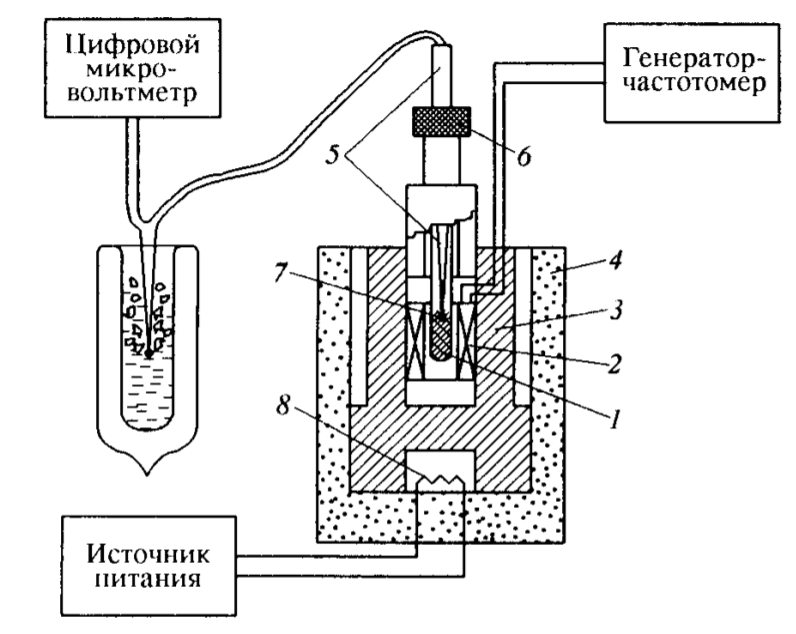
\includegraphics[width = 0.6\textwidth]{1.png}
\centering
\caption{Схема экспериментальной установки.}
\end{figure}


Магнитная восприимчивость образца определяется по изменению самоиндукции при его введению в катушку: пусть $L$ -- индуктивность с образцом, а $L_0$ -- без. Тогда
\[
L = \mu L_0,
\]
где $\mu$ -- магнитная проницаемость образца, то есть
\[
\dfrac{L - L_0}{L_0} = \dfrac{\Delta L}{L_0} = \mu - 1.
\]
Принимая в расчёт, что длина образца сильно больше его диаметра, можно пренебречь размагничивыющим фактором, тогда
\[
\dfrac{L - L_0}{L_0} = \dfrac{\Delta L}{L_0} = \mu - 1 = 4\pi \varkappa.
\]
С учётом того, что собственная частота контура обратно пропорциональна корню из индуктивности, получим
\begin{equation}\label{5}
\boxed{\dfrac{1}{\varkappa} \propto \dfrac{f^2}{f_0^2 - f^2}}
\end{equation}

\newpage
\section*{Выполнение и обработка данных}

Исследуем зависимость частот $f$ и $f_0$ от температуры, постепенно нагревая образец. Измерения  проводим в интервале от $10~^\circ \text{C}$ до $50~^\circ \text{C}$ с шагом в примерно $3~^\circ \text{C}$, результаты представлены в Таблице 1. В качестве погрешости выбираем последний знак отображаемого прибором числа, который стабилен.
\vspace{15pt}
\begin{figure}[h]
\begin{floatrow}
\ffigbox{%
  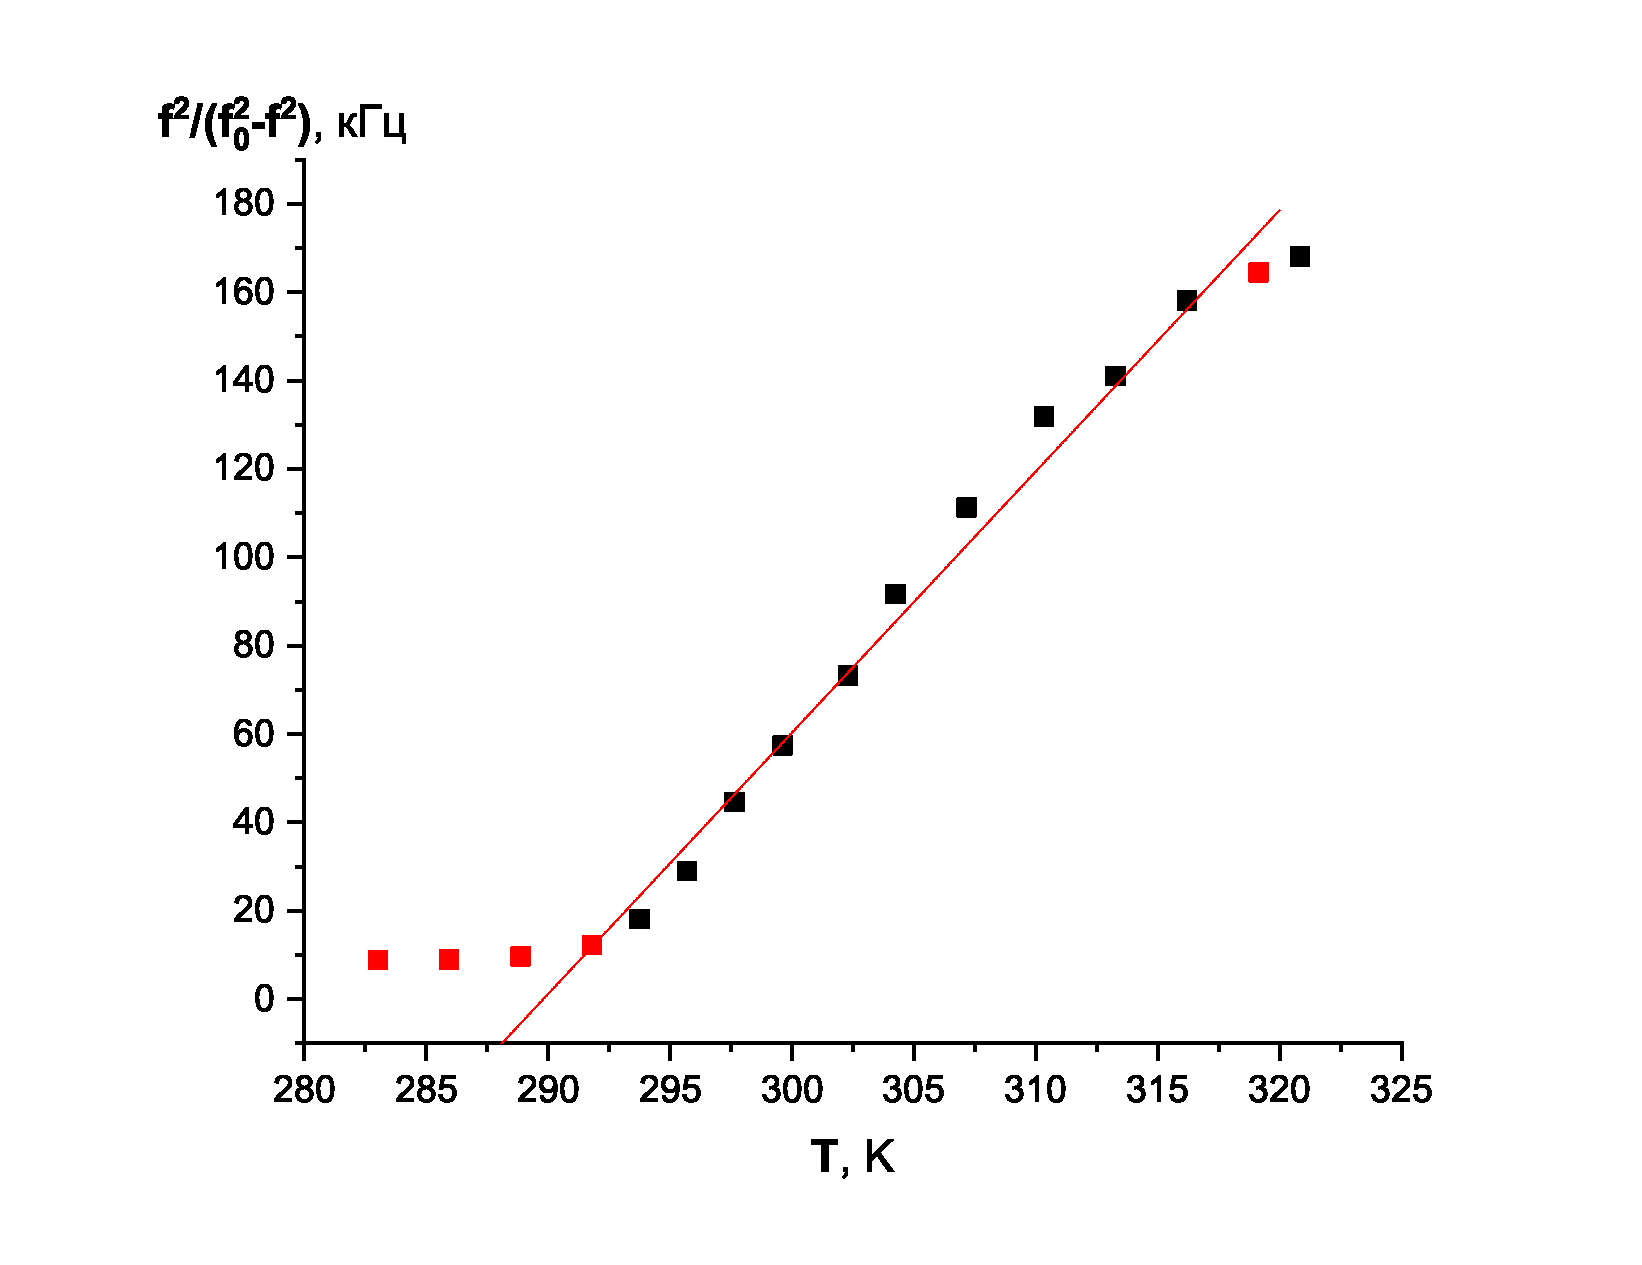
\includegraphics[width = 0.55\textwidth]{1.pdf}%
}{%
  \caption{Зависимость $\dfrac{f^2}{f_0^2-f^2}$ от $T$.}%
}
\capbtabbox{%
\vspace{-1cm}
\begin{tabular}{|c|c|c|c|c|}
\hline $U$, мВ & $T$, $^\circ \text{C}$ & $f$, кГц & $f_0$, кГц \\
\hline$-0.65$ & $9.88$  & $904.46$ & $953.75$  \\
\hline$-0.53$ & $12.80$  & $905.24$ & $954.01$  \\
\hline$-0.41$ & $15.73$  & $908.00$ & $953.85$  \\
\hline$-0.29$ & $18.66$  & $917.42$ & $953.91$ \\
\hline$-0.21$ & $20.61$  & $928.72$ & $953.93$ \\
\hline$-0.13$ & $22.56$  & $938.00$ & $954.03$  \\
\hline$-0.05$ & $24.51$  & $943.63$ & $954.14$  \\
\hline$0.03$ & $26.46$  & $945.89$ & $954.09$  \\
\hline $0.14$ & $29.15$  & $947.64$ & $954.09$   \\
\hline $0.22$ & $31.10$ & $948.88$ & $954.03$  \\
\hline $0.34$ & $34.02$  & $949.84$ & $954.10$  \\
\hline $0.47$ & $37.20$  & $950.47$ & $954.07$  \\
\hline $0.59$ & $40.12$  & $950.76$ & $954.12$  \\
\hline $0.71$ & $43.05$ & $951.05$ & $954.05$ \\
\hline $0.83$ & $45.98$  & $951.27$ & $954.16$  \\
\hline $0.90$ & $47.68$  & $951.46$ & $954.29$  \\
\hline
\end{tabular}
}{%
  \caption{Результаты измерений.}%
}
\end{floatrow}
\end{figure}\\
Результаты измерения изорбразим на графике (Рис. 2) в координатах $\left( T, \frac{f^2}{f_0^2-f^2}\right)$, линейный участок аппроксимируем прямой, угловой коэффициент наклона и начальная ординаты из метода наименьшних квадратов равны:
\[k = 5.9 \pm 0.3~\text{K}^{-1}.\]
\[b = -1710 \pm 80.\]
Пользуясь соотношениями (\ref{2}) и (\ref{5}), получаем
\[\Theta = -\dfrac{b}{k} = 290 \pm 20~\text{К}.\]
Пользуясь формулой (\ref{4}), оценим величину обменного интеграла, считая, что для гадолиния $n = 12$, $S = 7/2$:
\[J = 2.3 \pm 0.2~\text{K} = 0.198\pm 0.014~\text{мэВ}.\]
\section*{Обсуждение}
В ходе работы была исследована температурная зависимость магнитной восприимчивости гадолиния и определена температура Кюри $\Theta = 290 \pm 20~\text{К}$, что хорошо соответствует табличному значению $293.4~\text{К}$ из \cite{laba}. Тем не менее, по измеренным данным видно, что закон Кюри-Вейса не выполняется при температура, сильно отличающихся от $\Theta$. По полученному значению $\Theta$ был оценен обменный интеграл $J = 0.198\pm 0.014~\text{мэВ}$.


\begin{thebibliography}{9}
\bibitem{laba} 
Игошин Ф.Ф., Самарский Ю.А., Ципенюк Ю.М.
\textit{Лабораторный практикум по общей физики: Учеб. пособие для вузов. Т3. Квантовая физика.}. 
М.: Физматкнига - 2005.
\end{thebibliography}
\end{document}










